\documentclass[border=10pt]{standalone}
\usepackage{tikz}\usepackage{amsmath}\usetikzlibrary{arrows.meta,positioning}
\begin{document}
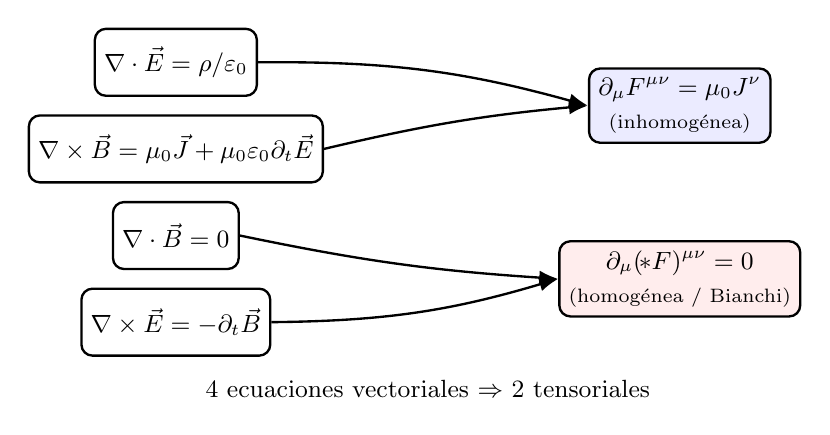
\begin{tikzpicture}[line width=0.85pt,>={Latex[length=2.4mm]},
   box/.style={draw,rounded corners,align=center,font=\small,minimum height=0.85cm}]
  \node[box] (g1) at (0,1.65) {$\nabla\cdot\vec E=\rho/\varepsilon_0$};
  \node[box] (g2) at (0,0.55) {$\nabla\times\vec B=\mu_0\vec J+\mu_0\varepsilon_0\partial_t\vec E$};
  \node[box] (g3) at (0,-0.55){$\nabla\cdot\vec B=0$};
  \node[box] (g4) at (0,-1.65){$\nabla\times\vec E=-\partial_t\vec B$};
  \node[box,fill=blue!8] (inh) at (6.4,1.1) {$\partial_\mu F^{\mu\nu}=\mu_0 J^\nu$\\[1pt]\scriptsize (inhomogénea)};
  \node[box,fill=red!7] (hom) at (6.4,-1.1){$\partial_\mu(\!*F)^{\mu\nu}=0$\\[1pt]\scriptsize (homogénea / Bianchi)};
  \draw[->] (g1.east) to[bend left=8] (inh.west);
  \draw[->] (g2.east) to[bend left=4] (inh.west);
  \draw[->] (g3.east) to[bend right=4] (hom.west);
  \draw[->] (g4.east) to[bend right=8] (hom.west);
  \node at (3.2,-2.5){\small 4 ecuaciones vectoriales $\Rightarrow$ 2 tensoriales};
\end{tikzpicture}
\end{document}
